\documentclass[10pt]{ctexart}
\usepackage{amsmath}
\usepackage{graphicx}
\usepackage{caption}
\title{迈克耳孙干涉仪实验报告}
\author{F组}
\pagestyle{empty}
\begin{document}
\maketitle
\section{实验原理}
\subsection{迈克耳孙干涉仪}
主要原理为光的分振幅干涉,使用分束镜将入射激光分为两束,经过反射后汇聚在光屏上,由于角度不同使得两束光的光程差在接收屏上改变,产生干涉条纹。

光强为$I=4I_0\cos^2(\frac{\Delta\phi}{2})$

又有$\Delta\phi=\frac{4\pi\Delta L}{\lambda}$

\[I=4I_0\cos^2(\frac{2\pi\Delta L}{\lambda})\]
$\Delta L$即为干涉仪两臂的长度差值

因此,干涉仪中心由明变暗或由暗变明一个周期需要移动的距离为$\frac{\lambda}{2}$

既可以通过已知的移动距离知晓光源的波长,又可以已知光源波长的情况下算出微小移动的距离
\subsection{测量光源相干性}
由于激光并非严格的单色光,因此激光干涉条纹会在明暗变化的同时整体产生衬比度的变化,有
\[\gamma=|\cos(\frac{\pi\Delta\lambda}{\lambda^2}\Delta L)|\]
可以通过观察条纹明显程度的变化来找到波长差
\subsection{测定折射率}
由于干涉仪的两臂之间的距离会影响条纹中心的明暗程度,因此可以通过其明暗变化来反映光程差的变化。考虑将待测玻璃块缓慢旋转来连续的改变光程差,用这种方法可以测量得到玻璃物块的折射率

通过折射定律$n\sin(\beta)=\sin(\alpha)$以及几何运算可得,由于玻璃物块而产生的光程变化为
\[\Delta L = 2(-\Delta L_1+nw+\Delta L_2 -nt)\]
因此折射率公式为
\[n=\frac{(\frac{N\lambda}{2t}+\cos\alpha-1)+\sin^2\alpha}{2(-\frac{N\lambda}{2t}-\cos\alpha+1)}\]
各项参数意义与图中相同
\begin{figure}
    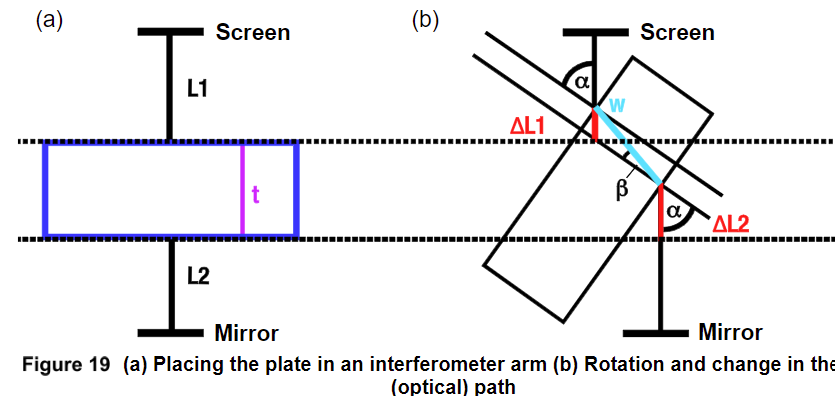
\includegraphics[width=0.8\textwidth]{折射率测定.png} 
    \caption{测定折射率实验原理}
\end{figure}
\subsection{测定热膨胀系数}
若已知光源波长,则可通过观察条纹吞吐个数来确定移动的距离.$\Delta L = \frac{N\lambda}{2}$

对于一根杆的热膨胀,近似遵循$\alpha=\frac{1}{L}\frac{dL}{dT}$

在温度变化较小的范围内$\Delta L\approx \alpha L_0 \Delta T$(此处$L_0$指杆的原始长度)

带入上式可得测量公式:
\[\rightarrow \alpha=\frac{N\lambda}{2L_0\Delta T}\]

\section{实验仪器与实验步骤}
\subsection{实验仪器}

\vspace{10pt}

\begin{minipage}{\textwidth} 
    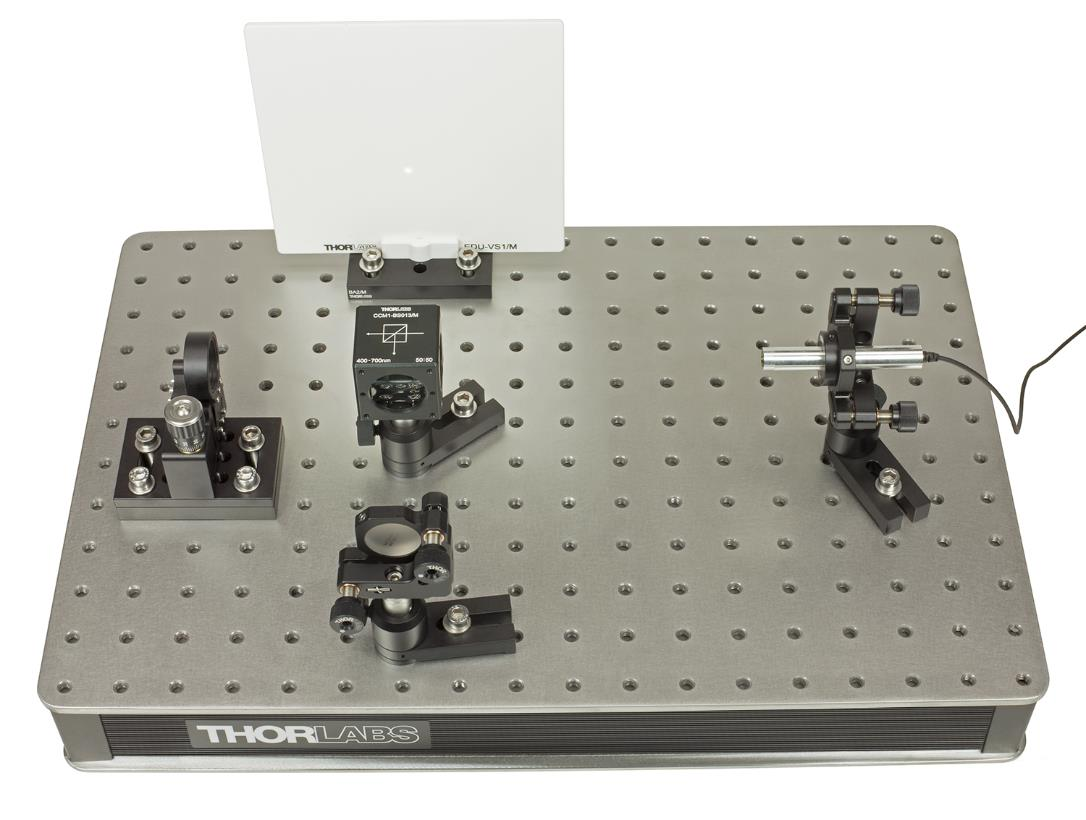
\includegraphics[width=0.8\textwidth]{基础光路图.jpg}
    \captionof{figure}{基础光路图}
\end{minipage}

\paragraph{干涉仪基本组件}

\begin{itemize}
    \item 钢制试验板
    \item 橡胶减震脚(我们使用的干涉仪由于底座重量不够,需要减震脚来使干涉仪保持尽量水平,尽管如此,对桌子的触碰按压依旧会带来影响)
    \item 准直激光二极管模块,532nm,二类,圆形光束(绿光清晰度高,便于观察)
    \item 电源
    \item 1英寸镜座*2
    \item 1英寸圆镜*2
    \item 塑料观察屏
    \item 1英寸双凸透镜,$f=50mm$(选择焦距为5厘米,大致是光具组的线度,便于调节产生平行光)
    \item 非偏振分光镜立方体(选择非偏振来使光源衬比度不因此下降)
\end{itemize}
\paragraph{折光率测量}
\begin{itemize}
    \item 高精度旋转支架(最小刻度为1/25度)
    \item 有机玻璃板 8mm,12mm(有机玻璃板的选取只需使转动过程中可覆盖激光即可)
\end{itemize}
\paragraph{LED实验组件}
\begin{itemize}
    \item 639nm发光二极管若干(发出红光)
    \item 白光发光二极管若干
    \item 尺子30cm(为了大致将光程调到相等)
\end{itemize}
\paragraph{热膨胀实验}
\begin{itemize}
    \item 1英寸铝镜
    \item 12.7mm、90mm长的铝杆,接头接受镜头支架
    \item 数字温度计(直接测量温度。分度值为0.1度,测量温度有滞后性)
    \item 加热器,带有十万欧姆电阻
\end{itemize}
\subsection{实验步骤}
\paragraph{激光波长的测定}\mbox{}

1.将可移动镜以及激光器置于试验板上。打开激光器并调整其方向使得由镜面反射回来的光斑正好落在激光器的出光孔中。另外,检查可动镜的旋钮是否太靠近其测量范围的边缘。

2.将分光镜按正确方向置于可动镜与激光器之间并将光屏置于分光镜出光侧,此时可以看到两个较亮的光斑,分别是在镜面上经过一次反射和两次反射产生的,缓慢转动分光镜使得两个光斑重合。此时有较暗的光斑与亮光斑不在一个高度上,这是由于装置各部分间存在对水平面的偏移。这个偏差对最后干涉条纹的实现影响不大,而且如果要进行消除会干扰原先已经调好的光路,影响装置稳定性,遂从略。

\begin{minipage}{\textwidth} 
    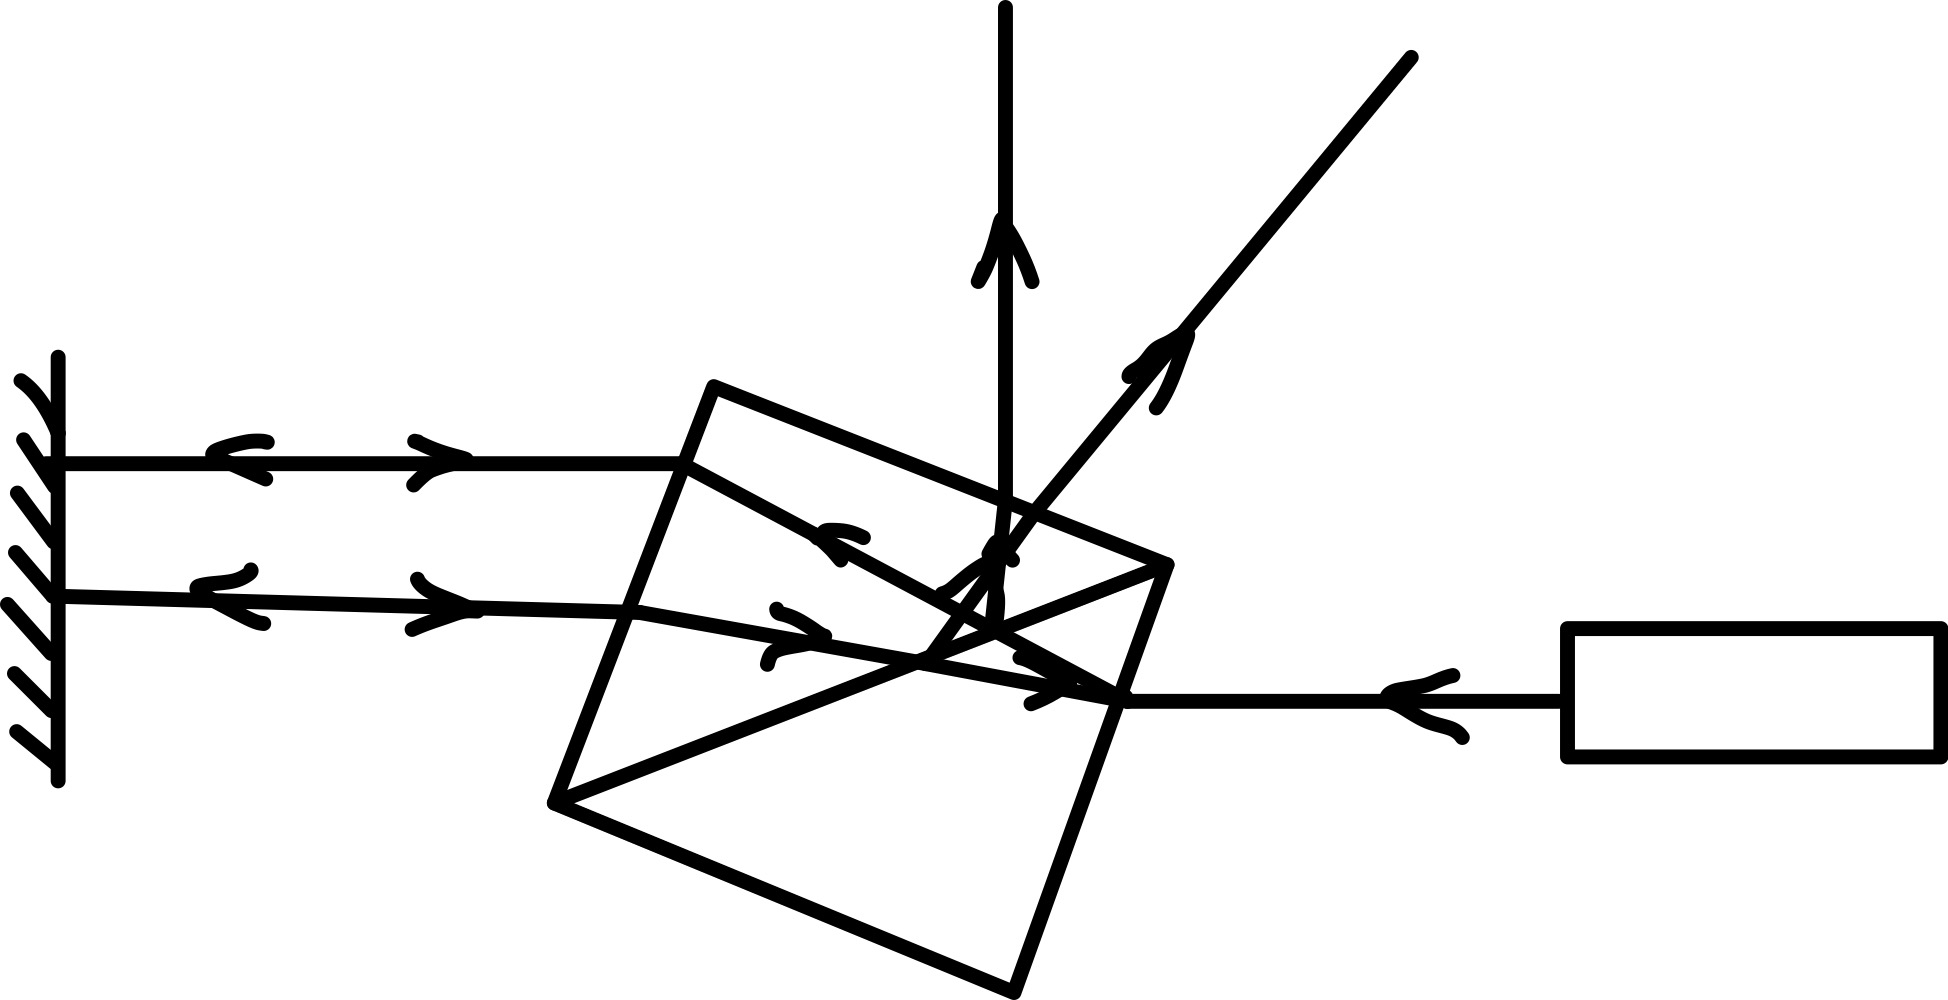
\includegraphics[width=0.8\textwidth]{两个光斑的解释.jpg}
    \captionof{figure}{两个光斑的解释}
\end{minipage}

3.在光屏对侧放置固定镜。为确保迈克尔逊干涉仪的两臂长度尽量相等,在摆放时应该尽可能确保此镜与分光镜的距离大致等于可动镜到分光镜的距离。此时在光屏上再次出现两个较大的光斑。转动反射镜使得光斑接近,再微调支架上的旋钮调整镜子角度使得光斑严格重合。此时,已经可以在光屏上看见干涉条纹。

4.在激光器和分光镜间放置透镜并调整其高度和角度使得在光屏上看见清晰的同心圆状的等倾干涉条纹。

\begin{minipage}{0.45\textwidth}
    \includegraphics[width=\textwidth]{等倾干涉条纹.jpg}
    \captionof{figure}{等倾干涉条纹}
\end{minipage}
\hfill
\begin{minipage}{0.45\textwidth}
    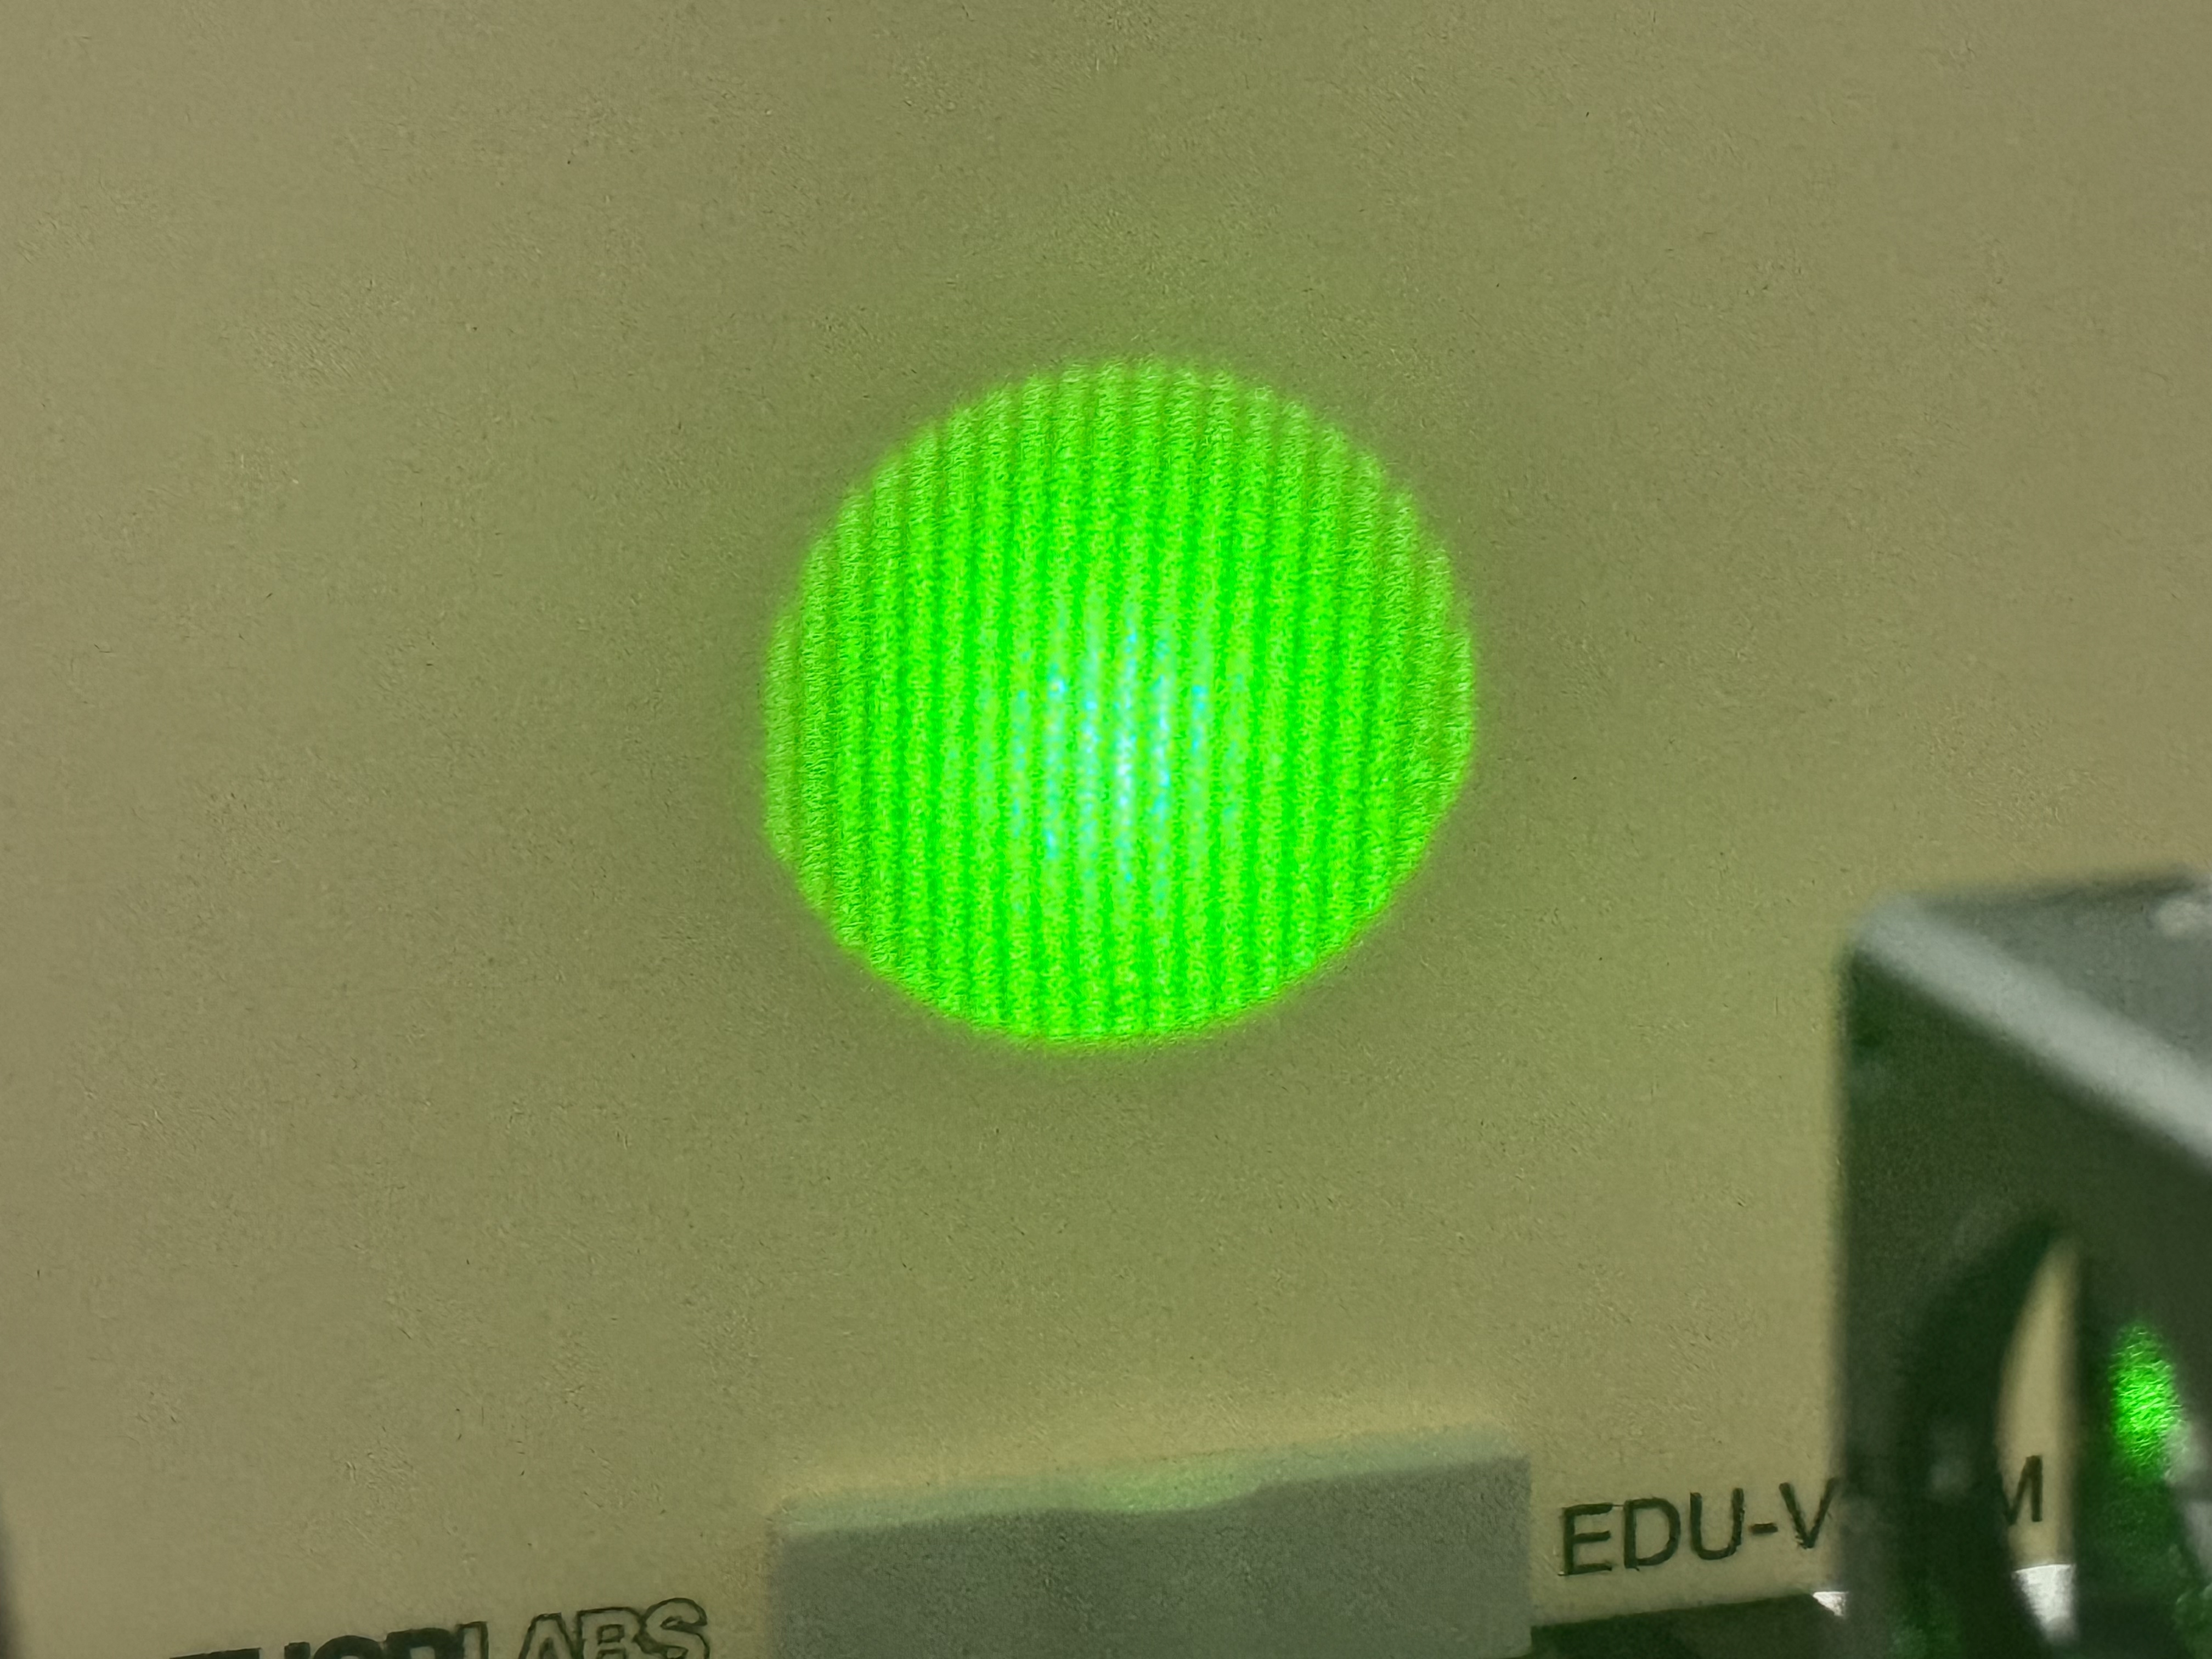
\includegraphics[width=\textwidth]{等厚干涉条纹.jpg}
    \captionof{figure}{等厚干涉条纹}
\end{minipage}

5.开始测量波长:向一个方向转动动臂的旋钮并计数条纹吞吐,每二十个计一次数,共计数12次。

6.演示实验:在动臂的下方,我们点亮了一个打火机,观察到原来的 等倾干涉图案发生了变化,类似于一块印有原来图案的橡胶膜受到了某些方向的应力作用后图案产生了畸变。

7.测量相干长度:在第一次实验中在条纹极细时没有观察到衬比度有明显变化,由于第一次实验现场有专业人士指导,经过我们的询问,以及他们的操作,给出的解释为由于实验所用激光器输出的激光接近于严格的单模,因此相干长度极长,在动臂的量程内未观测到衬比度的变化。测微器量程大概在几毫米,因此我们推测相干长度应大于毫米量级。在第二次实验中,我们将两臂光程差调到几乎一致,此时我们观察到了干涉条纹衬比度的变化,为此,我们产生了新的假想,记录于“讨论与心得”一节。

\begin{minipage}{0.45\textwidth}
    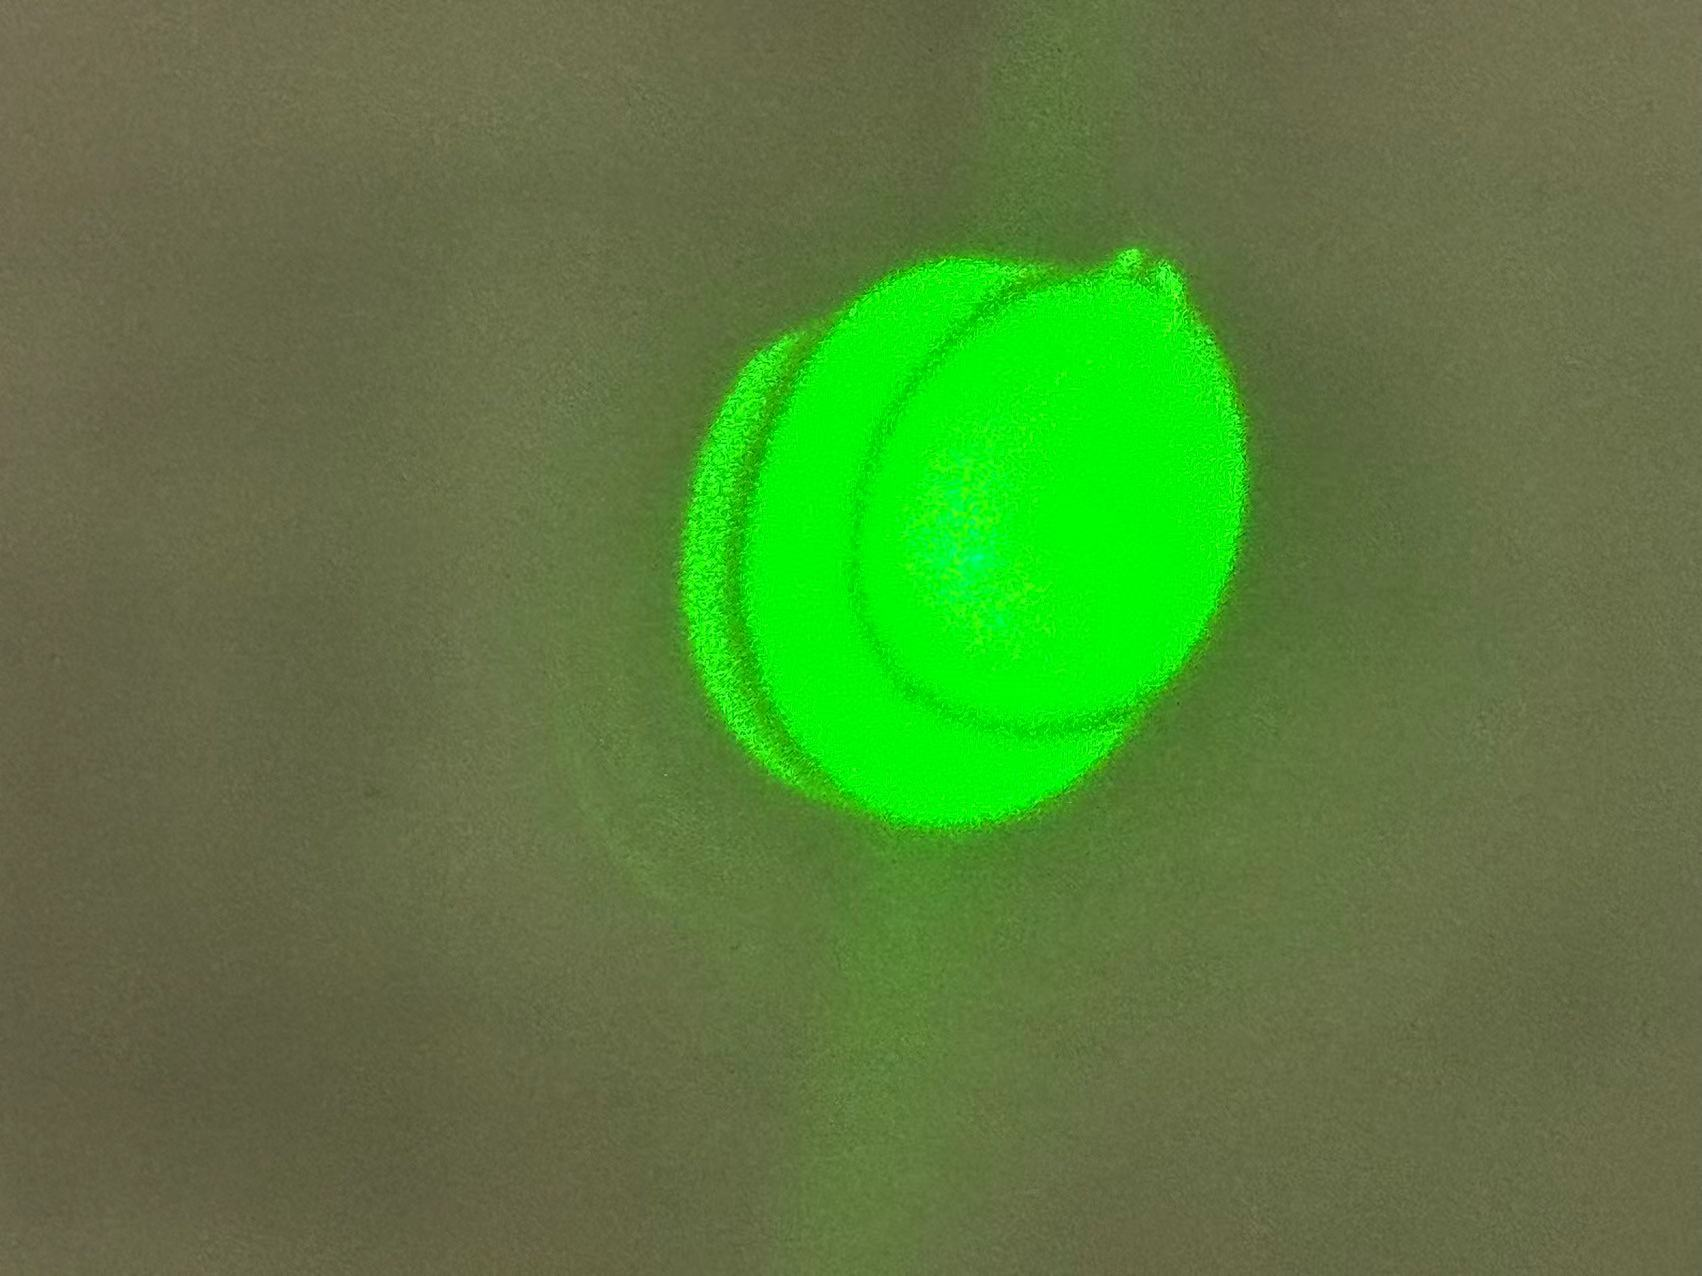
\includegraphics[width=\textwidth]{清晰.jpg}
    \captionof{figure}{清晰的条纹}
\end{minipage}
\hfill
\begin{minipage}{0.45\textwidth}
    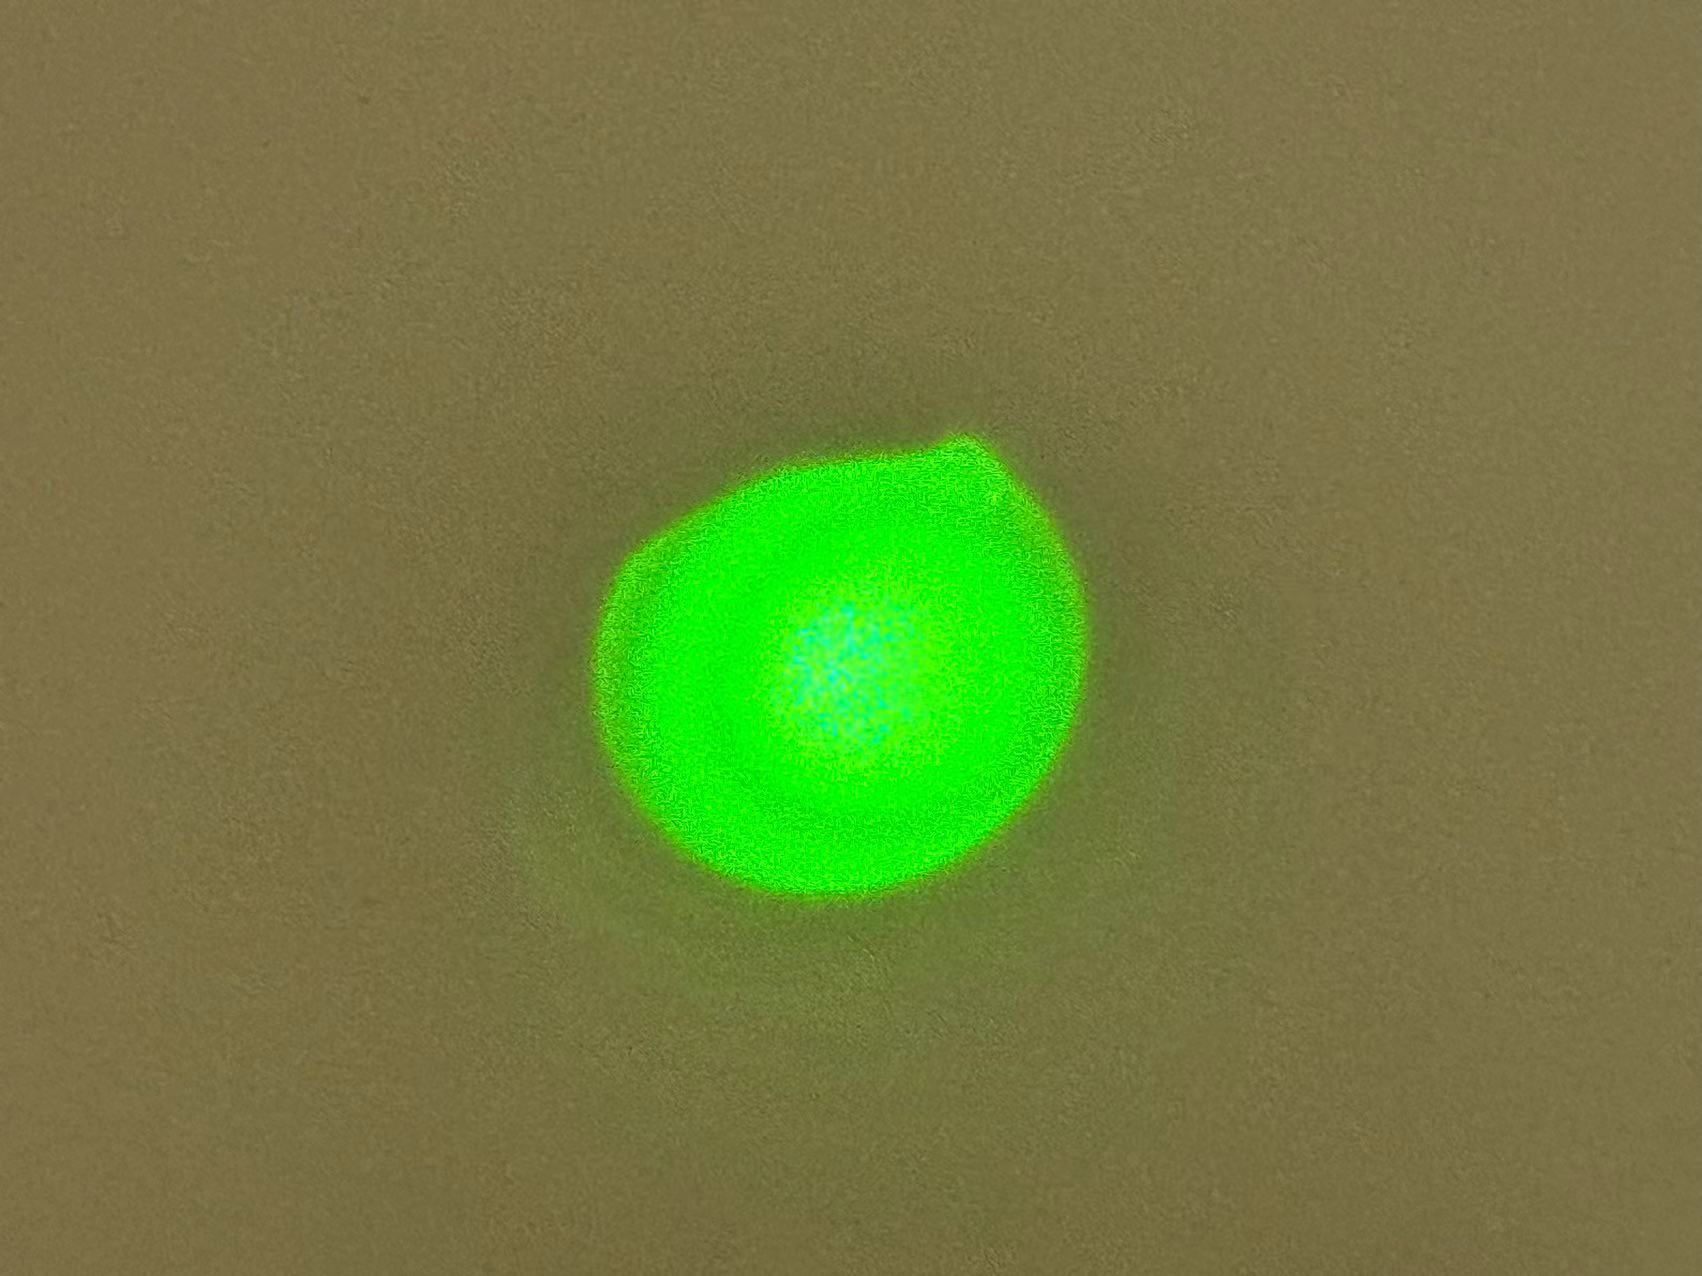
\includegraphics[width=\textwidth]{模糊.jpg}
    \captionof{figure}{模糊的条纹}
\end{minipage}

\paragraph{折射率的测定}\mbox{}

1.搭建迈克尔逊干涉仪,使光屏上可以观察到清晰的绿色条纹;

2.在其中一侧反射镜与分光镜之间放置玻璃板。粗调玻璃板位置,使目测下玻璃板法线几乎沿光路方向,拧紧螺丝以固定玻璃板位置;

3.旋转玻璃板底座的旋钮,以微调玻璃板角度,同时观察干涉条纹变化。找到条纹中心由“吞”到“吐”或由“吐”到“吞”的临界位置,此即玻璃板入射角为零的位置,记下此时的角度值;

4.从此位置开始,单向转动旋钮,同时观察条纹变化。条纹每吞(或吐)5次时,读出角度值并记录,直至累计到达85条;

5.数据处理,得出玻璃折射率。
\paragraph{热膨胀系数的测定}\mbox{}

1.将激光器及带有反射镜的杆置于试验板上。在杆中插入测温计枪头以时时测量杆的温度。调节反射镜角度,使激光器的反光正好打回激光器中心,此后保持杆的位置不变。

2.将分光镜按正确方向置于可动镜与激光器之间并将光屏置于分光镜出光侧,此时可以看到两个较亮的光斑。缓慢转动分光镜使得两个光斑重合。此时分光镜以调至合适角度,固定分光镜。

3.在光屏对侧放置固定镜。摆放时应该尽可能确保此镜与分光镜的距离大致等于可动镜到分光镜的距离。此时在光屏上再次出现两个较大的光斑。转动反射镜使得光斑接近,再微调支架上的旋钮调整镜子角度使得光斑严格重合。此时,已经可以在光屏上看见干涉条纹。

4.使用信号发生器对杆加热。通过选取不同的电压控制加热速率。先使杆升温至45℃,然后停止加热等待降温。一个同学盯紧温度计示数,另一个同学观察条纹吞吐圈数。每降低1℃,记下条纹吞吐数目,直至降温至35°C.

5.处理数据,得出杆的热膨胀系数。

\vspace{10pt}

\begin{minipage}{\textwidth} 
        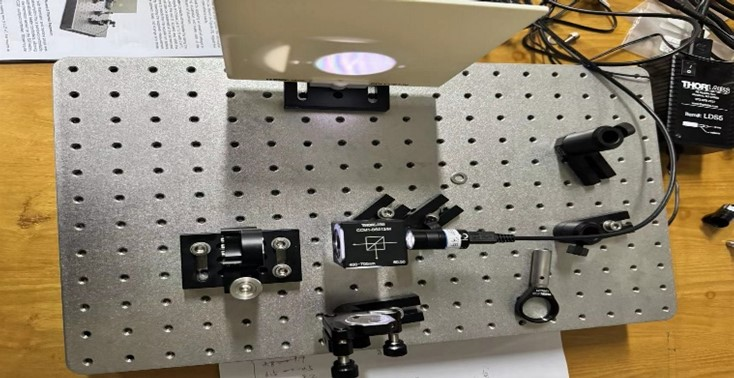
\includegraphics[width=0.8\textwidth]{图片1.jpg}
        \captionof{figure}{发光二极管作为光源的实验光路图}
\end{minipage}
\paragraph{LED干涉}
    

\begin{itemize}
    \item 红光LED
    1.调节两臂等长:先在绿激光下调出干涉条纹,并使两臂目测等长。此后,调节固定镜的前后距离,使条纹间距很大,并微调距离旋钮使得干涉仪不断吞入条纹。如图7所示。在此过程中,条纹间距继续增大,视场也会逐步偏离条纹中心。此时需要微调反光镜上的角度旋钮,使得视场尽可能接近条纹中心。尽管看不到中心,也要使得我们容易判断圆心在条纹的左还是右。然后,微调固定镜的距离旋钮,找到使得条纹弯曲方向由一侧转到另一侧的位置。我们的做法是取两个端点,即两端各取一个一定可以将条纹弯曲方向判定为“左”或“右”的位置,记下两端点读数,则两臂等长的位置一定在这两个位置之间。最后,取下激光,换上红光LED,使光源尽可能接近分光镜(如图6),在刚才确定的区间内调节距离旋钮,直至在光屏上观察到红光的干涉条纹。如图8.
    
    2.微调距离旋钮,使红光干涉条纹从模糊到清晰再到模糊,测出红光的极限相干长度。
    \item 白光LED
    将距离旋钮调至红光条纹最清晰处,取下红光,换上白光LED,即可观察到彩色的干涉条纹。如图9所示。同理测得白光的相干长度。
\begin{minipage}{0.35\textwidth}
        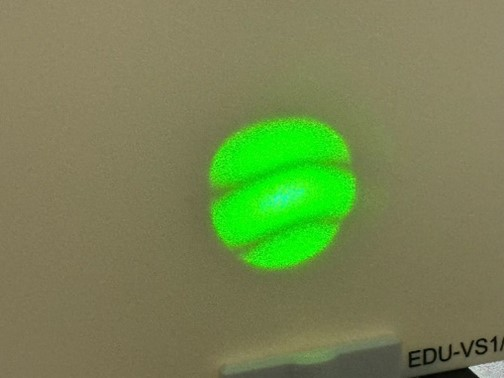
\includegraphics[width=\textwidth]{图片2.jpg}
        \captionof{figure}{绿光干涉的粗条纹}
    \end{minipage}
    \begin{minipage}{0.35\textwidth}
        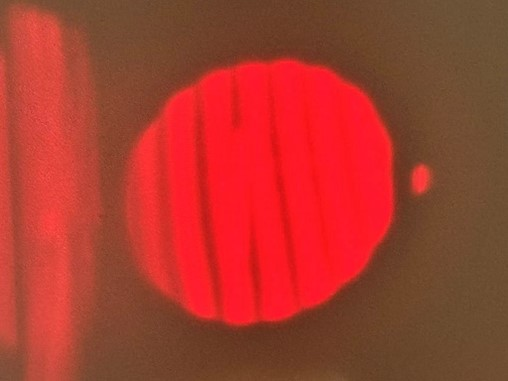
\includegraphics[width=\textwidth]{图片3.jpg}
        \captionof{figure}{红光干涉条纹}
    \end{minipage}
    \hfill
    \begin{minipage}{0.38\textwidth}
        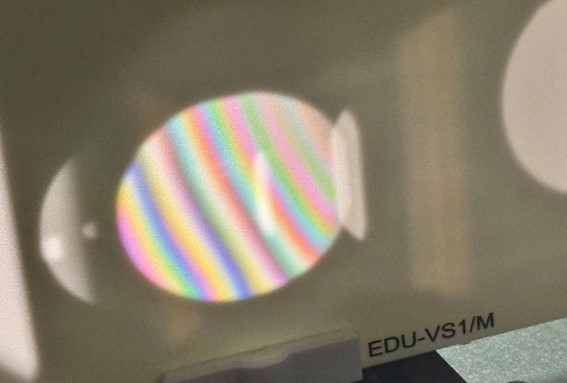
\includegraphics[width=\textwidth]{图片4.jpg}
        \captionof{figure}{白光干涉条纹}
    \end{minipage}
\end{itemize}
\paragraph{附}
在实验过程中发现分光镜上有指纹,在老师指导下进行了对光学镜面的擦拭

1.穿戴手套,注意不要触碰手指部分。

2.取出拭镜纸并折叠到合适大小并用镊子夹好,将拭镜纸用丙酮润湿,小心擦去光学面上的指纹。这是利用了丙酮对油脂有较强的溶解能力。

3.再取一张拭镜纸,重复步骤二以确保污渍被彻底清除

注意:由于丙酮有毒且挥发性强,最好在通风的地方完成这项操作。
\section{数据处理}
一、测量激光器波长

由前文实验原理,知:
\[I=4I_0\cos^2(\frac{2\pi\Delta L}{\lambda})\]

故有移动臂长$l_i$与条纹数$N_i$满足如下关系:
\[l_i=\frac{\lambda}{2} N_i+C\]

依据数据列表如下:
\begin{equation*}
    \begin{tabular}[c]{|c|c|c|}
        \hline
        条纹移动数$N_i$ & 测微器读数$l_i / 10^{- 6}$ & $(l_i - l_{i - 1}) / 10^{- 6}$ \\
        \hline 
        0 & 39.0 & / \\
        \hline
        20 & 44.6 & 5.6 \\
        \hline
        40 & 50.1 & 5.5 \\
        \hline
        60 & 55.8 & 5.7 \\
        \hline
        80 & 61.1 & 5.3 \\
        \hline
        100 & 66.0 & 4.9 \\
        \hline 
        120 & 71.2 & 5.2 \\
        \hline
        140 & 76.9 & 5.7 \\
        \hline
        160 & 82.3 & 5.4 \\
        \hline 
        180 & 87.9 & 5.6 \\
        \hline
        200 & 93.1 & 5.2 \\
        \hline
        220 & 98.2 & 5.1 \\
        \hline
    \end{tabular}
\end{equation*}

线性回归,\ 得:\ 
\begin{equation*}
    l = a N + b
\end{equation*}

其中:\ 
\begin{equation*}
    \left\{ 
        \begin{array}{l}
        a = 0.268776 \\
        b = 39.2846 \\
        r = 0.9999293
    \end{array} 
    \right.
\end{equation*}

\begin{equation*}
    \begin{array}{l}
        \sigma_y = 0.65 \\
        \sigma_a = 2.7 \times 10^{- 3}
    \end{array}
\end{equation*}

测微器允差:
0.004mm

故
\begin{equation*}
    \lambda = \frac{2 L}{N} + C
\end{equation*}

得:\ 
\begin{equation*}
    \lambda = (537 \pm 6) \text{nm}
\end{equation*}

二、确定热膨胀系数

公式:$\frac{1}{2}N\lambda=\alpha L_0 \Delta T$

获取数据:通过插在铝棒中的热电偶温度计测量温度,每隔1°C记下光屏中心吞吐的环数

数据处理:$\Delta T = \frac{\lambda}{2\alpha L_0}N$;对ΔT-N进行线性拟合。

\newpage


\section{实验分析讨论(心得体会)}
1.调整光路必须先弄清楚先后顺序。比如在最初调节光路时我们将所有的仪器摆放在实验台上调整,这样无法分清楚究竟应该调整那个仪器(因为就算是光斑重合,有可能是多个仪器的位置偏差导致误差相消),逐个调整仪器,有助于减少调整的自由度,降低调整的难度并避免因为多个仪器的偏差相消导致的假象。

2.在测量波长的过程中,一开始我们采用了分工的方法,一名同学转动旋钮调整臂长并读数,另一名同学数环数的吞吐。我们发现这样测量误差很大,与预期结果相去甚远。于是采取由同一名同学旋转旋钮并计数,这样可以避免眨眼导致错过环数,或者分不清楚具体出现的是一个还是两个环连续出现。

3.在调节迈克尔逊干涉仪时,注意到存在一个由四个螺丝固定的反射镜,此镜在固定后难以微调,故应先固定此镜,然后通过激光器在此镜的反射光去调节激光笔的倾角和位置,直至反射光打入激光笔中心;

4.迈克尔孙干涉仪是精度很高的仪器,但粗调在其中依旧具有非常重要的作用。在反复调节臂长等长的尝试中,我们发现,如果每次手动改变镜子位置后都使用最标准的办法,拿下扩束镜对合光斑,将会使实验过程非常繁琐,条纹粗细的变化也难以察觉。但我们发现,在首次调出条纹后,轻微改变镜子位置时,可以保留扩束镜,用手拿住镜子使其微小位移并时时微调,较易调出大间距的干涉纹。

5.关于极值的应用1:在进行迈克尔孙干涉实验时,存在很多零值的应用。比如在测量折射率时,要求我们测量玻璃的法线相对于光路的角度,这就需要先找到玻璃的法线与光线垂直的位置,一开始我们认为只需要目测调节就可以了,但在经过真正的测量后,我们发现一点小小的角度测量误差就可能会导致很大的偏移,尤其是数据较小时,所以我们在此处运用了极值进行调节。调节玻璃的角度来让条纹吞吐反向,此时光程取到极值,角度也刚好取到零。

6.测量折射率的实验中,在偏离角度较小时,一次吞吐所需的角度变化量极大,很容易因为这一点引起误差。我们在调节玻璃板法向与光线平行后,又调节了可移动的平面镜,使条纹恰好处于吞/吐临界点,这样就完美消除了初始条纹吞吐上的误差。

7.关于极值的应用2:在观察二极管的干涉时,也需要做到两臂尽可能等长,两臂等长时,不管朝哪个方向移动,都会使光程差变大,所以条纹反向时就是光程差为零时。然而,在等厚干涉的情况下,曲率半径趋近于正无穷,条纹吞吐难以观察,于是我们通过观察条纹弯曲方向来判断是否达到等光程点。亦即使用肉眼判断,圆心从右无穷远运动到左无穷远时,就是等光程点。

8.调节红光发光二极管干涉时,一开始在等光程点并不能够观察到干涉现象,后来,将红光二极管的方向转换后就又可以观察到干涉现象,且偏离角度不大于最大值时,偏离角度越大,干涉条纹衬比度越高,但偏离角度大于上述最大值后,衬比度再次减小。这可能是由于当垂直入射,发光二极管发出红光的发散角过大,导致有红光偏离迈克尔孙干涉仪,最后以不同的干涉图样照射在光屏上,遮盖了原有干涉条纹,所以减少进光量可以使发散角变小,几乎所有进入分束镜的光都能产生几乎相同的干涉条纹,于是衬比度得以上升。至于存在最大值,则是因为进入分束镜的光通量减少,肉眼分辨能力有限,加上环境光的干扰,最终导致衬比度下降。

9.我们在尝试测量激光器的相干长度时遇到了困难,激光器在接近等厚干涉时出现了条纹变得部分模糊的情况,但并没有完全消失,我们认为,可能是激光器的强度随波长的变化并不严格只有两个峰值,而是存在多个峰值,这样,我们观察到的模糊仅仅是其中一组干涉条纹相互干扰导致折射率部分下降。另外,也有可能是由于激光器光强在两个波长处并不是相等的,这也可以导致激光器虽然错开但衬比度仍然不能降到零的现象。
\end{document}


